%% LyX 2.2.2 created this file.  For more info, see http://www.lyx.org/.
%% Do not edit unless you really know what you are doing.
\documentclass[a4paper,english]{article}
\usepackage[T1]{fontenc}
\usepackage[latin9]{luainputenc}
\usepackage{array}
\usepackage{longtable}
\usepackage{url}
\usepackage{graphicx}
\usepackage{setspace}

\makeatletter

%%%%%%%%%%%%%%%%%%%%%%%%%%%%%% LyX specific LaTeX commands.
% Backwards compatibility for LuaTeX < 0.90
\@ifundefined{pageheight}{\let\pageheight\pdfpageheight}{}
\@ifundefined{pagewidth}{\let\pagewidth\pdfpagewidth}{}
\pageheight\paperheight
\pagewidth\paperwidth

%% Because html converters don't know tabularnewline
\providecommand{\tabularnewline}{\\}
%% A simple dot to overcome graphicx limitations
\newcommand{\lyxdot}{.}


%%%%%%%%%%%%%%%%%%%%%%%%%%%%%% Textclass specific LaTeX commands.
\newenvironment{lyxlist}[1]
{\begin{list}{}
{\settowidth{\labelwidth}{#1}
 \setlength{\leftmargin}{\labelwidth}
 \addtolength{\leftmargin}{\labelsep}
 \renewcommand{\makelabel}[1]{##1\hfil}}}
{\end{list}}

\makeatother

\usepackage{babel}
\begin{document}
\begin{center}

\includegraphics[scale=0.3]{images/Logo_Politecnico_Milano}
\par\end{center}

\begin{center}
Software Engineering 2 project:$\mathit{PowerEnJoy}$
\par\end{center}

\begin{spacing}{0}
\begin{center}
A.A. 2016/2017 - Prof. E. di Nitto
\par\end{center}
\end{spacing}

\vspace{20pt}
\begin{singlespace}
\begin{center}
\textbf{\huge{}RASD}
\par\end{center}{\huge \par}
\end{singlespace}

\begin{spacing}{0}
\begin{center}
\textbf{R}equirements \textbf{A}nalysis and \textbf{S}pecification
\textbf{D}ocument
\par\end{center}
\end{spacing}

\vspace{50pt}

Version \textbf{1.0 - }2016/11/02

\smallskip

\begin{tabular}{ll}
Pietro Avolio & Mat 878640\tabularnewline
Guido Borrelli & Mat XXXXXX\tabularnewline
\end{tabular}
\begin{center}
\newpage{}\tableofcontents{}
\par\end{center}

\newpage{}

\section{Introduction}

\subsection{Purpose}

ShareEnJoy is a new company that wants to enter the car sharing market
and wants to provide a service based on electric vehicles only.\\
The way they want to implement their service is classical and very
common to other car sharing services: it will be available in a specific
geographical area (called safe area) for each city where the service
will be activated. Users will be able to reserve and then rent a vehicle,
use it for as much time as they desire and then be charged based on
the rental time.

As the car sharing service is based on electric vehicles only, the
system must provide some specific functionalities in order to handle
electric vehicles behaviours and needs. For example, the company owns
some electric recharging stations spread among the safe area and users
should be encouraged to terminate their rentals in these stations.
\bigskip ShareEnJoy needs a digital management system in order to
support all the activities for both their customers and their operators. 

\subsection{Scope}

Following the ``The World \& Machine'' approach by M. Jackson and
P. Zave we can identify real word entities that interact with the
system (``the Word''), specific system entities (``the Machine'')
and the intersection beetwen them (``the shared phenomena'').
\begin{center}
\begin{figure}[h]
\begin{centering}
\includegraphics[scale=0.17]{\string"images/1.2 - The world and the machine - Page 1\string".png}
\par\end{centering}
\caption{``The World \& Machine'' Venn diagram}
\end{figure}
\par\end{center}

\pagebreak{}The system will be composed of three main modules with
different roles and purposes:
\begin{lyxlist}{00.00.0000}
\item [{$\mathit{ShareEnJoy~Mobile~App}$}] This component is intended
to be used by ShareEnJoy customers and will offer the functionality
to see available vehicles in a specific geographical area, to reserve
and then to rent a vehicle. It also allows users to unlock a reserved
vehicle when they're nearby Through the app users can also send support
requests to ShareEnJoy support staff.
\item [{$\mathit{ShareEnJoy~Control~Room}$}] This component is intended
to be used by ShareEnJoy operators in order to have a real time blueprint
of the system, to handle support requests and to be notified for some
specific events (e.g. an automatic payment failure, a car that runs
out of battery).
\item [{$\mathit{ShareEnJoy~Core}$}] This component is intended to contain
all the system logic. It should work as a connection node between
all the other components as well as connection point to vehicles.
It should handle user\textquoteright s payments through a payment
gateway and perform automated tasks.
\end{lyxlist}
A list of high level goals that the system should accomplish is the
following:
\begin{lyxlist}{00.00.0000}
\item [{|G1|}] The system should know vehicles position and information
such as model, battery percentage, mechanical issues and damages.
\item [{|G2|}] The system should be able to show on a map the position
of available vehicles together with some selected status information
(e.g. battery percentage) and estimated information (e.g. kilometers
authonomy). 
\item [{|G3|}] Users should be able to register and insert a payment method.
\item [{|G4|}] Users should be able to reserve a vehicle, unlock it when
they\textquoteright re close to it's position and start the rent. 
\item [{|G5|}] The system should charge the users after each rent with
fees based on company policies.
\item [{|G6|}] Users should be able to send a support request.
\item [{|G7|}] Company operators should be able to handle support requests
forwarded by users.
\item [{|G8|}] Company operators should be able to see and handle notifications
sent by the system.
\end{lyxlist}

\subsection{Definitions, acronyms and abbreviations}

In order to avoid ambiguity and possible misunderstanding here are
formally listed some recurrent terms and acronyms used in this document. 

\begin{longtable}[l]{|l|>{\raggedright}p{0.73\columnwidth}|}
\hline 
The System & The digital management system to be developed.\tabularnewline
\hline 
ShareEnJoy & The company to develop the system for. Also referred as 'the company'.\tabularnewline
\hline 
Vehicle & A vehicle owned by the company that can be used in the car sharing
service.\tabularnewline
\hline 
User & A person who wants to use the system and it's not a member of the
company.\tabularnewline
\hline 
Logged-in user & A user who has completed the log-in process so that it can be associated
with a real identity and payment information.\tabularnewline
\hline 
Customer & A user or a logged-in user.\tabularnewline
\hline 
Operator & A person who wants to use the system and it's authenticated as a member
of the company.\tabularnewline
\hline 
Availabe vehicle & A vehicle that is not reserved by anywan and can be reserved by a
logged-in user.\tabularnewline
\hline 
Reserved vehicle & A vehicle that has been reserved by a logged-in user.\tabularnewline
\hline 
Rented vehicle & A vehicle that is currently rented by a logged-in user.\tabularnewline
\hline 
Expired reservation & A reservation that has not been cancelled or transformed in a rental
after a certain amount of time defined by company policies.\tabularnewline
\hline 
Safe Area & The geographical area in which a vehicle can be parket and rental
terminated.\tabularnewline
\hline 
DBMS & Database Management System\tabularnewline
\hline 
TBD & To Be Determined\tabularnewline
\hline 
\end{longtable}

\subsection{Reference documents}
\begin{lyxlist}{00.00.0000}
\item [{|REFD1|}] Assignments AA 2016-2017
\item [{|REFD2|}] ISO/IEC/IEEE 29148, first edition, 2011-12-01
\item [{|REFD3|}] Requirements Engineering Part III
\item [{|REFD4|}] IDC Research Inc analysis on mobile operating systems
market share~\url{http://www.idc.com/prodserv/smartphone-os-market-share.jsp},
2016 Q2
\item [{|REFD5|}] Android distribution per version~\url{https://developer.android.com/about/dashboards/index.html},
as of 2016-11-02
\item [{|REFD6|}] iOS per version distribution~\url{https://david-smith.org/iosversionstats/},
as of 2016-11-02
\end{lyxlist}

\subsection{Overview}

TODO

\newpage{}

\section{Overall Description}

\subsection{Product perspective}

The central component of the entire system is the ShareEnJoy Core
module which is where all the logic is put. This module of the system
is in charge of providing an interface to vehicles on-board information
system, of processing requests from the other modules of the system,
of accessing system database and of interfacing with the payment gateway.

\bigskip

All the other modules of which the system is made of (i.e. ShareEnJoy
Mobile App and ShareEnJoy Control Room) should interface with the
core module in order to accomplish required tasks (e.g. user\textquoteright s
registration and login, vehicle reservation request, etc).
\begin{center}
\begin{figure}[h]
\begin{centering}
\includegraphics[scale=0.8]{\string"images/RASD 2.1 - Product Prospective - Page 1\string".png}
\par\end{centering}
\caption{Block diagram of the system structure}
\end{figure}
\par\end{center}

\subsubsection{User Interfaces}
\begin{lyxlist}{00.00.0000}
\item [{$\mathit{ShareEnJoy~Mobile~App}$}] This module will be implemented
as a mobile application and it's intended for costumers. It's important
that the most used commands are visibile and easy navigable. Secondary
commands of less frequent usage can be organised in secondary less
visible menus.\bigskip In order to avoid mistakes between commands
it's better to not have too many selection on every page, text explainations
should be clear and concise. Error windows should show short error
descriptions together with an error identification code.\bigskip
The application should follow the design guidelines of the different
operating system it will be implemented for (i.e. Material design
for Android, ModernUI for iOS) and support all screen resolutions
between ldpi and xxdpi.\\
\begin{figure}[h]
\begin{centering}

\includegraphics[scale=0.7]{Mockups/App/Landing}\hspace{10pt}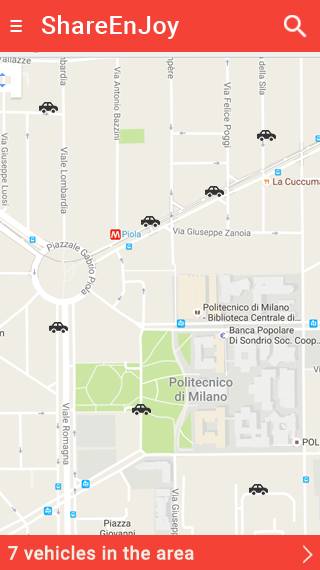
\includegraphics[scale=0.7]{Mockups/App/Map}\\
\hspace{10pt}
\par\end{centering}
\begin{centering}
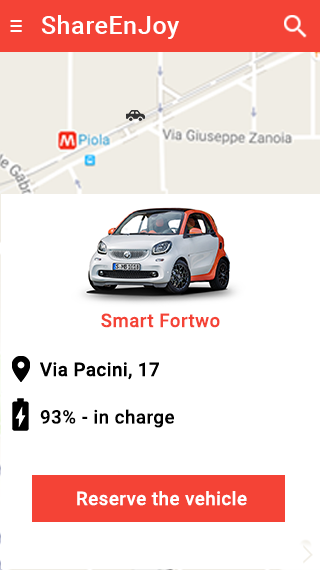
\includegraphics[scale=0.7]{Mockups/App/Vehicle_detail}\hspace{10pt}\includegraphics[scale=0.7]{\string"Mockups/App/Vehicle Reserved\string".png}
\par\end{centering}
\caption{ShareEnJoy Mobile App mockups}

\end{figure}
\item [{$\mathit{ShareEnJoy\,Control\,Room}$}] This module will be implemented
as a web application and it is intended for operators. Functionalities
should be well categorized and unambiguous. Most frequently used functions
should be as easy and immediate as possibile in order to speed-up
operators work and reduce customers wait time. Some macros could be
present in order to reduce repetitve tasks. It should be accesible
through a common internet connection and it should be well optimized
for a single chosen browser and a screen resolution. Error windows
should show a long error message in order to easily recover.
\item [{$\mathit{ShareEnJoy\,Core}$}] This module does not provide a direct
user interface since it's intended to be managed and maintained by
qualified and specialized staff. It should provide a very detailed
activity logs.
\end{lyxlist}

\subsubsection{Hardware interfaces}
\begin{lyxlist}{00.00.0000}
\item [{$\mathit{ShareEnJoy\,Mobile\,App}$}] This component should obtain
device location by its operating system. If GPS position is unavailable
or insufficiently precise, a localization through wifi network could
be possibile. If both methods fail or can't provide the desired level
of acuracy the application can't work properly.
\item [{$\mathit{ShareEnJoy\,Control\,Room}$}] This software does not
have any hardware interfaces.
\item [{$\mathit{ShareEnJoy\,Core}$}] This software does not have any
hardware interfaces.
\end{lyxlist}

\subsubsection{Software interfaces}
\begin{lyxlist}{00.00.0000}
\item [{$\mathit{ShareEnJoy\,Mobile\,App}$}] Android and iOS together
cover about the 99\% of the mobile operating system market share\footnote{REFD4}
and are the systems we are going to focus on.\\
After analysing per operating system distribution and share, a good
compatibility tradeoff could be the following.\\
\\
\begin{tabular}{|l|l|}
\hline 
\multicolumn{2}{|c|}{Mobile device operating system}\tabularnewline
\hline 
Operating System & Min. version\tabularnewline
\hline 
Android & 4.1 (API level 16)\tabularnewline
\hline 
iOS & 9\tabularnewline
\hline 
\end{tabular}\\
\\
With this minimal requirements we can support 97\% of android devices\footnote{REFD5}
and 92\% of iOS devices\footnote{REFD6}
\item [{\pagebreak{}}]~
\item [{$\mathit{ShareEnJoy\,Control\,Room}$}] This software will require
a Java EE application server. It should integrate a support ticket
system in order to handle support requests forwarded by users.\\
\\
\begin{tabular}{|l|l|}
\hline 
\multicolumn{2}{|c|}{Application server}\tabularnewline
\hline 
Name & Glassfish\tabularnewline
\hline 
Version & 4.1.1\tabularnewline
\hline 
\end{tabular}\hspace{10pt}%
\begin{tabular}{|l|l|}
\hline 
\multicolumn{2}{|c|}{Support ticket system}\tabularnewline
\hline 
Name & osTicket\tabularnewline
\hline 
Version & OSE 1.10\tabularnewline
\hline 
\end{tabular}
\item [{\label{ShareEnJoyCore_Required_Softwares}$\mathit{ShareEnJoy\,Core}$}] This
software has to interface with vehicles on-board information system,
with the payment gateway and with a DBMS. It will require a Java EE
application server.\\
\\
\begin{tabular}{|l|l|}
\hline 
\multicolumn{2}{|l|}{Vehicles information system}\tabularnewline
\hline 
Name & ShareEnJoy Vehicle I.S.\tabularnewline
\hline 
Version & 1.0\tabularnewline
\hline 
\end{tabular}\hspace{10pt}%
\begin{tabular}{|l|l|}
\hline 
\multicolumn{2}{|l|}{Payment Gateway}\tabularnewline
\hline 
Name & GESTPAY\tabularnewline
\hline 
Version & Professional\tabularnewline
\hline 
\end{tabular}\\
\\
\begin{tabular}{|l|c|}
\hline 
\multicolumn{2}{|l|}{DBMS}\tabularnewline
\hline 
Name & MySql Community Edition\tabularnewline
\hline 
Version & 5.7.6\tabularnewline
\hline 
\end{tabular}\hspace{10pt}%
\begin{tabular}{|l|l|}
\hline 
\multicolumn{2}{|c|}{Application server}\tabularnewline
\hline 
Name & Glassfish\tabularnewline
\hline 
Version & 4.1.1\tabularnewline
\hline 
\end{tabular}\\
\\
The module can properly work on every operating system as long as
these components are installed and work properly.
\end{lyxlist}

\subsubsection{Communication Interfaces}

All modules should communicate with the core module in order to complete
tasks, thus the core module can be seen as an internal API provider.
All the communications between the modules are bidirectional and could
be implemented through the internet HTTPs protocol using a REST approach.
Responses could be in the JSON format.

\begin{figure}[h]
\begin{centering}
\includegraphics[scale=0.17]{\string"images/RASD 2.1.5 - Communication interfaces - Page 1\string".png}
\par\end{centering}
\caption{System modules communication scheme}

\end{figure}

Communication between the core and the DBMS works using the TCP protocol
on port 3306.

Communication between the core and the payment gateway works using
the TCP protocol on an arbitrary port.

The ShareEnJoy control room can be accessed using the HTTPs protocol
on port 80.

\subsubsection{Memory constraints}

Users must have enough space to install ShareEnJoy Mobile App application
on their own devices. The size of the application is still unknown
but it can be estimated in less than 100MB.\bigskip

The system on which the core module will be run requires enough primary
memory space in order to install required softwares (section \ref{ShareEnJoyCore_Required_Softwares}).
Other 5GB of primary memory space are required for the database and
the software itself.\\
A good amount of secondary memory (i.e. 32GB) will result in better
performances for both the software itself and the DBMS.

\subsubsection{Operations}

TODO

\newpage{}

\subsection{Product functions}

In this section are listed all the functionalities that the system-to-be
is going to provide.

\subsubsection{Functional requirements}

Functional requirements are listed per system module:
\begin{lyxlist}{00.00.0000}
\item [{$\mathit{ShareEnJoy~Mobile~App}$}]~
\begin{itemize}
\item Registration
\item Log-in
\item See and edit logged-in user's own profile information and payment
method
\item Show available vehicles on map
\item Search available vehicles based on GPS localization or specific address
\item Show vehicle information (i.e. battery percentage, estimated kilometers
authonomy)
\item Make new or cancel existent vehicle reservation
\item Unlock a reserved vehicle
\item Guide the user to the reserved vehicle
\item Send a support request
\end{itemize}
\item [{$\mathit{ShareEnJoy\,Control\,Room}$}]~
\begin{itemize}
\item Operators login
\item Show all vehicles position and information
\item Show user's account information, disable an user
\item Show user's last activities
\item Show users' support requests and allow operators to reply or close
the requests
\item Show system notifications and mark them has $\mathit{handling}$,
$\mathit{handled}$, $\mathit{not-handled}$
\item Mark a vehicle as $\mathit{unavailable}$ (e.g. when the vehicle has
a mechanical issue)
\item Charge users for driving fines.
\end{itemize}
\item [{$\mathit{ShareEnJoy\,Core}$}]~
\begin{itemize}
\item Handle rent events (i.e. $\mathit{RENT\,STARTED}$, $\mathit{RENT\,TERMINATED}$)
\item Send commands to vehicles (e.g. $\mathit{UNLOCK\,DOORS}$)
\item Charge users after each rent applying company pricing policies
\item Handle payment failure: disable the user'acount if it's payment information
are nomore valid
\item Access and edit the company database
\item Notify users via SMS on their mobile phone number or via push notifications
through the SharEnJoy Mobile App
\item Generate monthly invoices and sent them to the users on their email
address
\item Detect expired reservation and charge the user for them
\end{itemize}
\end{lyxlist}

\subsubsection{Non-functional requirements}
\begin{itemize}
\item The system must be able to handle thousands of requests simultaneously.
\item The system should work properly 24 hour a day, 7 days a week and should
provide an high uptime score. Maintenance can be scheduled during
the night, when traffic is lower.
\item Users' information should be securely stored in the company database
and not accessible to unhautorized people. Espacially passwords should
be encryptet using efficient cryptography algorithms.
\end{itemize}

\subsubsection{Company pricing policies}

The company has defined some specific pricing policies to be applied
in correspondence with some specific user behaviours
\begin{itemize}
\item Expired reservation has a cost of 1EUR.
\item The rental starts as the user turns on vehicle engine.
\item The rental stops as the user parks the vehicle within the safe area
and all the passengers leave the vehicle.
\item Rental fee is per minute.
\item A 10\% discount is applied on the total rental fee if there are at
least 2 other passengers in the vehicle for more than the 50\% of
the rental time.
\item A 20\% discount is applied on the total rental fee if the vehicle
is parked with more than 50\% of battery capacity available.
\item A 30\% discount is applied on the total reantl fee if the vehicle
is parked in a charging station and the user plugs-in the charging
cable.
\item A 30\% extra fee is applied on the total rental fee if the vehicle
is left more than 3KM away from a rechargin station or if the vehicle
is left with less than 20\% of battery capacity available.
\item If more than a discount or an extra fee should be applied, extra fees
are applied first in ascendant order, discounts are applied later
in descendant order.
\end{itemize}

\subsection{User characteristics}

We distinguish beetwen two main categories of users
\begin{lyxlist}{00.00.0000}
\item [{$\mathit{ShareEnJoy\,Customers}$}] Customers that want to use
the service in order to rent a vehicle.
\begin{itemize}
\item Users: They can only see the position of available vehicles. Anyone
that uses the app without logging-in.
\item Logged-in users: They can access to all the functionalities of the
service. They are associated with a real identity and a payment method.
Logged-in users should possess a valid driving license, which should
be indicated during the registration process. People with disabilities
that doesn't allow the to drive a normal vehicle cannot register and
use the service: this check is done validating drive license data
during the registration process.
\end{itemize}
\item [{$\mathit{ShareEnJoy\,Operators}$}] They are workers of the company,
thus they have a good knowledge about the service and will follow
a training on how to use ShareEnJoy Control Room software.
\end{lyxlist}

\subsection{Constraints}

\subsubsection{Regulatory policies}

The system needs to store in the company database customers' personal
information (e.g. name, surname, address, email address, telephone
number) as well as to access users' locations in order to track vehicles.
Sensible data treatment should respect local laws belonging to each
area where the service will be available.

\subsubsection{Safety and security considerations}

Communications between system modules should be secure and use latest
encryption protocol in order to avoid man-in-the middle or other kind
of informatic attacks that could lead to data loss.\\
Communications towards vehicles should be secured in order to avoid
illegal vehicles unlocks perfomerd by malicious users or other types
of illegal behaviours.

\subsection{Assumptions and dependencies}

The system is based on the following domain assumptions:
\begin{itemize}
\item Information provided by vehicles on-board information systems (i.e.
vehicle location provided by
\item GPS, battery percentage, mechanical damages) are always available
and accurate.
\item If a vehicle cannot obtain location by GPS or has not internet connection
it is considered unavailable and not shown to users.
\item Vehicles always unlock when the system tells them to unlock. This
is true for each type of command.
\item Vehicles on-board information systems are always able to detect and
provide: battery percentage, number of passengers, mechanical failures,
GPS location.
\item If a user has a valid driving license then he can access the service
(this mainly deals with disabilities).
\end{itemize}

\subsection{Further developments}
\begin{itemize}
\item Allow the creation of different user groups in order to have different
system behaviours based on the group (e.g. different pricing policies
for groups).
\item Allow the creation of coupons that users can use to have special discounts.
\end{itemize}
\newpage{}

\section{Specific requirements}

\subsection{Functional requirements}

\subsubsection{Scenarios}

In order to better describe functional requirements listed in section
2.2.1 here is a list of possible system usages (scenarios) from various
viewpoints

\paragraph{$\mathrm{Scenario\,}1$ User registration and log-in\protect \\
}

Luca is a university student who moved to Milan for studying. He can\textquoteright t
afford to buy a car but sometimes he needs to move even when public
transports are unavailable (i.e. during the night ). He decided to
try a car sharing service and downloaded ShareEnJoy Mobile App in
order to use it during the incoming weekend. Once the download is
complete and the app is installed on his smartphone, Luca starts the
registration process: first he needs to create an account filling-in
his name and email address, his mobile phone number and choosing an
username. Email address is not yet used and username is available,
thus he can continue inserting his driving license ID: he missed a
characters so the application shows an error message. Luca fixes the
mistake and moves on to the latest step in which he is requested to
insert his credit card information. A fee of 0,01EUR is charged on
his credit card in order to validate it and the registration process
is complete.\\
Luca receives on his email address his password and can now log-in.

\paragraph{$\mathrm{Scenario}\,2$ Search for a vehicle and make a reservation\protect \\
}

Martin is a business man and he is just landed to Milan Malpensa airport.
He is going to have an intensive day and he needs to move fast in
the town center. He is taking a train from Malpensa to Stazione Centrale
station and during the 30 minutes time trip he plans to reserve a
vehicle near Stazione Centrale in order to do not waste time when
he will get off the train. He is a ShareEnJoy user and he starts the
application on his smartphone: he fills in the address and sees available
vehicles on the map. He founds a vehicle with enough power according
to his requirements and 3 minutes walking from the station. He decides
to reserve the vehicles and clicks the relative button on the application.
Now Martin can relax until he reaches Stazione Centrale.

\paragraph{$\mathrm{Scenario}\,3$ Unlock a vehicle and start the rent\protect \\
}

Marco is walking home after his evening gym session when he spots
a ShareEnJoy car parked along the street. He is tired by his training
session so he decides to check if the car is available. Marco starts
the application on his smartphone and checks for available vehicles
nearby using his GPS location. The vehicle along the street is available
so Marco reserves it and, being less than 5 meters away from the car,
he is able to unlock it using the relative button on the application.
Marco jumps in the car, secures the fast belt and starts the engine:
the rental starts and the price to be paied is shown on the screen
installed in the car. 

\paragraph{$\mathrm{Scenario}\,4$ User terminates a rent\protect \\
}

Mario and his friends are planning to go the the cinema tonight but
the place they want to reach is not covered by city public transports.
Mario is an old ShareEnJoy customer and he knows that the place is
inside the safe area and that ShareEnJoy applies a special discount
on the rental fee if there are passengers. He rents a vehicle and
reaches the cinema: once there, he stops the engine and terminates
the rent. An SMS sent to his mobile phone number informs him of the
final price, which was influenced by a number of company policies.
9EUR is the base price, plus he has got a 10\% discount because he
traveled with friends, a 20\% discount because he left the car with
more than 50\% of the battery capacity available and a 30\% extra
fee because there are no recharging station in a 3KM range from the
cinema. Mario thinks that 8,43EUR is a very good price to spent a
cinema night with friends (with which he will divide the cost later!).

\paragraph{$\mathrm{Scenario}\,5$ User sends a support request and operator
handles it\protect \\
}

Mario had a really busy day and he is now looking for an available
ShareEnJoy car so that he can reach his friends at the restaurant.
Mario uses the application on his smartphone to reserve a vehicle
but when he reaches the car he has an unexpected surprise: the car
has no wheels because they have been stolen. He uses the application
to open a support request describing the problem. The operator sees
the request in the ShareEnJoy Control Room software and gives instruction
on what to do to the client. Then, he marks the car as unavailable
and sends a notification to the mechanics team.

\paragraph{$\mathrm{Scenario\,6}$User tries to terminate the rent outside a
safe area\protect \\
}

Marta is new to the car sharing services and it is the first time
she rents a ShareEnJoy vehicle. She wants to reach Rho, a town near
Milan, but it is outside the safe area and she has not read information
documents. Once she reaches her destination, she stops the engine
and tries to terminate the rent: a message on the screen installed
in the car and an SMS sent to her mobile phone number notifies her
that she can't terminate the rent in that location and that she will
be charged until she will terminate the rental inside the safe area.
Marta checks the map and starts the engine again in order to move
the car inside the safe area, which is just 700mt away from her destination.

\paragraph{$Scenario\,7$ User's payment fails\protect \\
}

Carol has just terminated a rental but she has no left money on her
prepayed credit card. As soon as the ShareEnJoy Core Module tries
to make a payment and it is refused, it disables Carol's account and
sents her a notification both via SMS and email. She will not be ablo
the use her account to rent a vehicle until she will update her payment
information and pay the given amount.

\paragraph{$\mathit{Scenario\,8}$ User took a driving loan\protect \\
}

A driving loan has just been received at the ShareEnJoy headquarter.
The operator takes the loan and just inserts the amount and the date
with the time in the ShareEnJoy Control Room software. The system
automatically charges the user who was driving the vehicle in that
specific time. The user is notified via both SMS and email.
\end{document}
